\documentclass[12pt, a4paper]{article}

\usepackage{amsmath, amssymb, amsfonts}
\usepackage{float}
\usepackage{graphicx}
\usepackage{listings}
\usepackage{xcolor}
\usepackage[linesnumbered, ruled]{algorithm2e}
\usepackage{subcaption}
\usepackage[hidelinks]{hyperref}
% Each algorithm is written twice: the algorithm2e block (what the PDF typesets)
% and a plain-text Verbatim block right after it (what the web shows — pandoc
% renders Verbatim as a copyable <pre> code block). \excludecomment makes pdflatex
% SKIP the Verbatim blocks, so the PDF shows only the algorithm2e version; pandoc
% conversely drops each algorithm2e to an (empty, CSS-hidden) div and keeps the
% Verbatim. Because pdflatex never sees the Verbatim, its Unicode maths glyphs
% (⟨⟩ ← τ ∈ ∞ …) need no inputenc/literate setup.
\usepackage{comment}
\excludecomment{Verbatim}

\definecolor{codegreen}{rgb}{0,0.6,0}
\definecolor{codegray}{rgb}{0.5,0.5,0.5}
\definecolor{codepurple}{rgb}{0.58,0,0.82}
\hypersetup{linktoc=all}

\lstset{
    language=Python,
    basicstyle=\ttfamily\small,
    keywordstyle=\color{blue},
    commentstyle=\color{codegreen},
    stringstyle=\color{codepurple},
    breaklines=true,
    numbers=left,
    numberstyle=\tiny\color{codegray},
    frame=single,
    showstringspaces=false
}

\title{AI Masterclass Test 1}
\author{}
\date{}

\begin{document}

\maketitle
\tableofcontents

\newpage

\section{Problem Formulation}

\noindent A problem, $\mathcal{P}$, is defined by the following elements:

\[
\mathcal{P} = \langle S, s_0, A, \tau, c, G \rangle
\]

\noindent where:
\begin{itemize}
    \item $S$ is the state space
    \item $s_0 \in S$ is the initial state
    \item $A = \{a_1, \dots, a_k\}$ is set of actions or operations
    \item $\tau : S \times A \to S$ is the state transition function
    \item $c : S \times A \times S \to \mathbb{R}$ is the cost function
    \item $G \subseteq S$ defines the goal to be achieved.
\end{itemize}

\noindent A solution 
\[
\vec{a} = (a_0, a_1, \dots, a_n) \in \text{soln}(\mathcal{P})
\]
which induces a state sequence
\[
(s_0, s_1, \dots, s_{n+1})
\]
has an associated cost:
\[
c(\vec{a}) = \sum_{i=0}^{n} c(s_i, a_i, s_{i+1})
\]

\noindent A solution $\vec{a}^*$ is \textbf{optimal} if it minimises corresponding cost:
\[
\vec{a}^* \in \arg \min_{\vec{a} \in \text{soln}(\mathcal{P})} c(\vec{a})
\]

\section{State Transition Graph}
\begin{figure}[H]
    \centering
    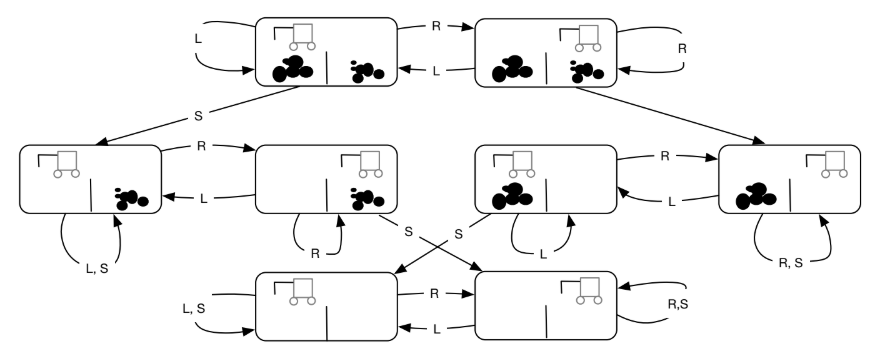
\includegraphics[width=0.9\textwidth]{images/state_transition_graph.png} 
    \caption{State transition graph with valid states and transition/actions}
    \label{fig:my_handwritten_notes}
\end{figure}

\bigskip

\textbf{Defining state vector in Code}\newline

\begin{lstlisting}[]
class VacuumWorldState:
    def __init__(self, 
                 dirtLeft=True, 
                 dirtRight=True, 
                 robotLeft=True):
        self.dirtLeft = dirtLeft
        self.dirtRight = dirtRight
        self.robotLeft = robotLeft

    def robotRight(self):
        return not self.robotLeft
\end{lstlisting}

\section{Breadth First Search}
\begin{algorithm}[H]
% \caption{BFS}
\SetKwFunction{Fbfs}{bfs}
\SetKwProg{Fn}{function}{}{end function}
\Fn{\Fbfs{$\mathcal{P} = \langle S, s_0, A, \tau, c, G \rangle$}}{
    $agenda \leftarrow newQueue()$\;
    $agenda.enQueue(s_0)$\;
    \While{not agenda.isEmpty()}{
        $s \leftarrow agenda.deQueue()$\;
        \tcp{expand s}
        \For{$a \in A$}{
            $s' \leftarrow \tau(s, a)$\;
            \If{$s' \in G$}{
                \tcp{goal found?}
                \Return "done"\;
            }
            \tcp{goal not found so add s' to queue}
            $agenda.enQueue(s')$\;
        }
    }
}
\end{algorithm}
\begin{Verbatim}
function bfs(P = ⟨S, s₀, A, τ, c, G⟩):
    agenda ← newQueue()
    agenda.enQueue(s₀)
    while not agenda.isEmpty():
        s ← agenda.deQueue()          # expand s
        for a ∈ A:
            s' ← τ(s, a)
            if s' ∈ G:                # goal found?
                return "done"
            agenda.enQueue(s')        # goal not found, add s' to queue
\end{Verbatim}

\begin{itemize}
    \item Utilise queue for FIFO
    \item Expand all nodes on depth $n$ before expanding any on depth $n+1$.
    \item For $b$ the branching factor and $d$ the depth at which the solution occurs,
    then BFS takes $O(b^d)$ (i.e. explores $1 + b + b^2 +\ldots + b^d$).
\end{itemize}

\noindent Evaluation
\begin{itemize}
    \item Completeness: BFS guaranteed to find a solution if it exists.
    \item Time complexity: is exponential in depth of the tree. If solution at shallower depths, BFS is good approach.
    \item Space complexity: Requires storing at least entire frontier of $b^d$. Susceptible to combinatorial explosion for larger problems.
    \item Optimality: Solution found will be optimal.
\end{itemize}

\newpage

\section{Depth First Search}
\begin{algorithm}[H]
% \caption{DFS}
\SetKwFunction{Fdfs}{dfs}
\SetKwProg{Fn}{function}{}{end function}
\Fn{\Fdfs{$\mathcal{P} = \langle S, s_0, A, \tau, c, G \rangle$}}{
    $agenda \leftarrow newStack()$\;
    $agenda.push(s_0)$\;
    \While{not agenda.isEmpty()}{
        $s \leftarrow agenda.pop()$\;
        \tcp{expand s}
        \For{$a \in A$}{
            $s' \leftarrow \tau(s, a)$\;
            \If{$s' \in G$}{
                \tcp{goal found?}
                \Return "done"\;
            }
            \tcp{goal not found so add s' to stack for evaluation}
            $agenda.push(s')$\;
        }
    }
}
\end{algorithm}
\begin{Verbatim}
function dfs(P = ⟨S, s₀, A, τ, c, G⟩):
    agenda ← newStack()
    agenda.push(s₀)
    while not agenda.isEmpty():
        s ← agenda.pop()              # expand s
        for a ∈ A:
            s' ← τ(s, a)
            if s' ∈ G:                # goal found?
                return "done"
            agenda.push(s')           # goal not found, add s' to stack
\end{Verbatim}

\begin{itemize}
    \item Utilise stack for LIFO
    \item Expands one branch at a time till the deepest node
\end{itemize}

\noindent Evaluation
\begin{itemize}
    \item Completeness: Not guaranteed to find a solution if one exists
    \item Time complexity: If it finds a solution, it takes much less time than BFS
    \item Space complexity: Current branch - $d$ nodes at depth $d$.
    \item Optimality: Solution found not guaranteed to be optimal.
\end{itemize}

\newpage

\section{Depth Limited Search}
\begin{algorithm}[H]
% \caption{Depth-Limited Search (DLS)}
\SetKwFunction{Fdls}{DLS}
\SetKwProg{Fn}{function}{}{end function}
\Fn{\Fdls{$\mathcal{P} = \langle S, s_0, A, \tau, c, G \rangle, limit \in \mathbb{N}$}}{
    $depth(s) \leftarrow 0$ for all $s \in S$\;
    $agenda \leftarrow newStack()$\;
    $agenda.push(s_0)$\;
    \While{not agenda.isEmpty()}{
        $s \leftarrow agenda.pop()$\;
        \For{$a \in A$}{
            $s' \leftarrow \tau(s, a)$ // expand s\;
            \If{$s' \in G$}{
                \Return "done"\;
            }
            $depth(s') \leftarrow depth(s) + 1$\;
            \If{$depth(s') \leq limit$}{
                $agenda.push(s')$ // goal not found\;
            }
        }
    }
    \Return "no solution"\;
}
\end{algorithm}
\begin{Verbatim}
function DLS(P = ⟨S, s₀, A, τ, c, G⟩, limit ∈ ℕ):
    depth(s) ← 0  for all s ∈ S
    agenda ← newStack()
    agenda.push(s₀)
    while not agenda.isEmpty():
        s ← agenda.pop()
        for a ∈ A:
            s' ← τ(s, a)              # expand s
            if s' ∈ G:
                return "done"
            depth(s') ← depth(s) + 1
            if depth(s') ≤ limit:
                agenda.push(s')       # goal not found
    return "no solution"
\end{Verbatim}

\begin{itemize}
    \item DFS might not terminate if it expands wrong branch with no solution on it.
DLS imposes some depth limit on exploring branches.
\end{itemize}

\newpage

\section{Iterative Deepening}
\begin{algorithm}[H]
% \caption{Iterative Deepening (ID)}
\SetKwFunction{Fid}{ID}
\SetKwProg{Fn}{function}{}{end function}

\Fn{\Fid{$\mathcal{P} = \langle S, s_0, A, \tau, c, G \rangle$}}{
    $limit \leftarrow 1$\;
    \While{true}{
        \If{DLS($\mathcal{P}, limit$) == "done"}{
            \tcp*[h]{goal found?} \;
            \Return "done"\;
        }
        \Else{
            $limit \leftarrow limit + 1$\;
        }
    }
}
\end{algorithm}
\begin{Verbatim}
function ID(P = ⟨S, s₀, A, τ, c, G⟩):
    limit ← 1
    while true:
        if DLS(P, limit) == "done":   # goal found?
            return "done"
        else:
            limit ← limit + 1
\end{Verbatim}

\begin{itemize}
    \item If we only perform DLS until depth $d$, but the solution is found at $d+1$, 
    we never find the solution.
    \item Iterative Deepening repeats DLS (calls DLS as subroutine) at increasing depths till solution is found.
    \item We need to regenerate nodes up till depth $d-1$ when we do DLS for depth $d$.
    \item This is tradeoff of time for memory.\newline
    \textbf{Example} $b=10$, $d=5$. BFS would require examining 111,111 nodes, with memory requirement of 100,000 nodes.
    Iterative deepening search 123,456 nodes, with memory requirement of only 50 nodes. Takes 11\% longer with 2000\% reduction in memory.
\end{itemize}

\newpage

\section{Bi-directional search}
\begin{itemize}
    \item Search from goal state backwards as well as initial state forwards. Each direction can use different search strategies.
    \item Involves iteratively determining predecessor nodes to goal, and those before it.
    \item Performs two $b^{d/2}$ searches instead of one $b^d$ search.
    \item \textbf{Example} For $b=10$, $d=6$, BFS examines 1,000,000 nodes, while Bidrectional search examines 2,000 nodes.
\end{itemize}If $d$ is large, it it still impractical.

\newpage

\section{Uniform Cost Search}
\begin{algorithm}[H]
% \caption{Uniform Cost Search (UCS)}
\SetKwFunction{Fucs}{UCS}
\SetKwProg{Fn}{function}{}{end function}

\Fn{\Fucs{$\mathcal{P} = \langle S, s_0, A, \tau, c, G \rangle$}}{
    $g(s) \leftarrow \infty$ for all $s \in S$\;
    $agenda \leftarrow \{s_0\}$ \tcp*[r]{agenda is a set}
    \While{$agenda \neq \emptyset$}{
        $C \leftarrow \arg \min_{s \in agenda} g(s)$\;
        $s' \leftarrow$ any element of $C$\;
        \If{$s' \in G$}{
            \tcp*[h]{goal found?} \;
            \Return "done"\;
        }
        \For{$a \in A$}{
            \tcp*[h]{expand s} \;
            $s'' \leftarrow \tau(s', a)$\;
            update $g(s'')$ -- replace existing value if smaller\;
            $agenda \leftarrow agenda \cup \{s''\}$\;
        }
    }
}
\end{algorithm}
\begin{Verbatim}
function UCS(P = ⟨S, s₀, A, τ, c, G⟩):
    g(s) ← ∞  for all s ∈ S
    agenda ← {s₀}                     # agenda is a set
    while agenda ≠ ∅:
        C ← arg min_{s ∈ agenda} g(s)
        s' ← any element of C
        if s' ∈ G:                    # goal found?
            return "done"
        for a ∈ A:                    # expand s
            s'' ← τ(s', a)
            update g(s'')  (replace existing value if smaller)
            agenda ← agenda ∪ {s''}
\end{Verbatim}

\begin{itemize}
    \item We have the cost function
    \[c: S \times A \times S \rightarrow \mathbb{R}\]
    \item UCS involves keeping cost of the path to any node. Let this be $g(s) \in \mathbb{R}$.
    \item UCS utilises a priority queue, where the priority is the path cost.
    \item UCS expands cheapest nodes first (in order of incerasing path cost).
    \item Always finds optimal path if costs are non-negative ($\implies$ path costs either stay the same or increase). 
    If UCS found the goal with cost $C$,
    there can't be another path with cost $C' < C$, since UCS would already have expanded the path,
    by definition of the priority queue.
    \item UCS becomes BFS when all step costs are equal.
\end{itemize}

\begin{figure}[H]
    \centering
    % --- Left Column (Image) ---
    \begin{minipage}{0.45\textwidth}
        \centering
        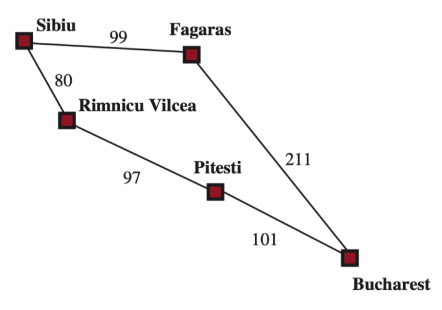
\includegraphics[width=\textwidth]{images/ucs-eg.png}
        \caption{Handwritten diagram}
    \end{minipage}
    \hfill % Adds horizontal space between the two columns
    % --- Right Column (Text/Code) ---
    \begin{minipage}{0.45\textwidth}
    Execution Example
    \begin{itemize}
    \item Successors are Rimnicu (80) and Fagaras (99)
    \item Rimnicu is selected for expansion
    \item Successor is Pitesi ($80 + 97 = 177$)
    \item Least cost is now Fagaras
    \item Successor is Bucharest ($99 + 211 = 310$)
    \item Pitesi now selected for expansion
    \item Bucharest updated ($80 + 97 + 101 = 278$)
    \item Bucharest selected for expansion; goal reached with optimal path
    \end{itemize}    
    \end{minipage}
\end{figure}

\newpage

\section{Greedy Search}

\begin{algorithm}[H]
% \caption{Greedy Search}
\SetKwFunction{Fgreedy}{greedy}
\SetKwProg{Fn}{function}{}{end function}

\Fn{\Fgreedy{$\mathcal{P} = \langle S, s_0, A, \tau, c, G \rangle$}}{
    $agenda \leftarrow \{s_0\}$ \tcp*[r]{agenda is a set}
    \While{$agenda \neq \emptyset$}{
        $C = \arg \min_{s \in agenda} h(s)$\;
        $s' \leftarrow$ any element of C\;
        \For{$a \in A$}{
            $s'' \leftarrow \tau(s', a)$\;
            \If{$s'' \in G$}{
                \tcp*[h]{goal found?} \;
                \Return "done"\;
            }
            \tcp*[h]{goal not found so add $s''$ to agenda} \;
            $agenda \leftarrow agenda \cup \{s''\}$\;
        }
    }
}
\end{algorithm}
\begin{Verbatim}
function greedy(P = ⟨S, s₀, A, τ, c, G⟩):
    agenda ← {s₀}                     # agenda is a set
    while agenda ≠ ∅:
        C ← arg min_{s ∈ agenda} h(s)
        s' ← any element of C
        for a ∈ A:
            s'' ← τ(s', a)
            if s'' ∈ G:               # goal found?
                return "done"
            agenda ← agenda ∪ {s''}   # goal not found, add s'' to agenda
\end{Verbatim}

\begin{itemize}
    \item We have seen $g(s)$, the path cost \textit{to} some node.
    \item Heuristics estimate cost of cheapest path \textit{from} some node to the solution.
    \[h: S\rightarrow \mathbb{R}\]
    Heuristics should be cheap to compute, otherwise we just use the resources to search.
    \item Greedy search expands node with cheapest expected cost ($h(s)$) to solution.
    \item Greedy search is an informed version of DFS; both focus on one path.
    \item Just like DFS, greedy search does not guarantee the optimal solution. 
    It is myopic as it ignores how expensive it was to reach a node.
\end{itemize}

\newpage

\section{A* Search}
Minimises both path cost so far \textit{and} estimated cost to goal,
\[f(s) = g(s) + h(s)\]

\paragraph{Admissible heuristics} A heuristic function is admissible (optimistic) if
it never overestimates the true cost to the goal.
\[0\leq h(s) \leq h^*(s), \quad \forall s\]
where $h^*(s)$ is the true lowest cost to from $s$ to the goal.

\paragraph{Theorem} If $h(s)$ is admissible, A* is guaranteed to find an optimal path to the goal.\newline 
Because A* never overestimates, A* never ignores a shorter path in favour of a longer one. 
So when A* reaches the goal for the first time, it is guaranteed to be the optimal one.


\paragraph{Example} 2D grid: Manhatten distance (for strictly vertical and horizontal movements)
\[h(s) = |x_s - x_g| + |y_s - y_g|\]
where $(x_s, y_s)$ is coordinate of state $s$ and $(x_g, y_g)$ is coordinate of goal state.\newline
The actual steps needed is at least equal to the number of horizontal steps + vertical steps.

\paragraph{Example} Unrestricted movement in 2D space: Euclidean distance
\[h(s) = \sqrt{(x_s - x_g)^2 + (y_s - y_g)^2}\]

\paragraph{Example} 8-puzzle
\begin{figure}[H]
    \centering
    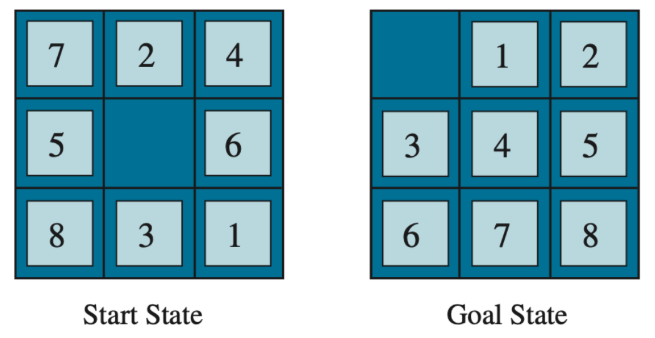
\includegraphics[width=0.5\textwidth]{images/8-puzzle.png} 
    \caption{$h(s)$ = number of misplaced tiles or sum of Manhatten distances of each tile to their goal position}
    \label{fig:my_handwritten_notes}
\end{figure}

\newpage

\section{Comparison of searches}
\begin{table}[h]
\centering
\begin{tabular}{|l|l|l|l|}
\hline
\textbf{Strategy} & \textbf{Selection from frontier} & \textbf{Path found} & \textbf{Space} \\ \hline
{\color{blue} Breadth-first} & First node added (FIFO) & Fewest arcs & $O(b^d)$ \\ \hline
{\color{blue} Depth-first} & Last node added (LIFO) & $\times$ & $O(bd)$ \\ \hline
{\color{blue} Iterative deepening} & N/A & Fewest arcs & $O(bd)$ \\ \hline
{\color{red} Uniform cost} & Minimal $c(p)$ & Least cost & $O(b^d)$ \\ \hline
{\color{red} Greedy} & Minimal $h(p)$ & $\times$ & $O(b^d)$ \\ \hline
{\color{red} A*} & Minimal $c(p) + h(p)$ & Least cost & $O(b^d)$ \\ \hline
\end{tabular}

\vspace{1em}
\small
\begin{tabular}{c}
$b$ = branching factor \\
$d$ = depth of shallowest solution \\
$\times$ = not guaranteed to find solution \\
{\color{blue} blue} = uninformed, {\color{red} red} = informed
\end{tabular}
\end{table}

\newpage

\section{Game Trees - Backward Induction}

\begin{algorithm}[H]
\caption{Zermelo's Algorithm}
\DontPrintSemicolon

$done \leftarrow leaves((S, E))$\;
\While{$done \neq S$}{
    $next \leftarrow \{s' \in S \setminus done \mid children(s', (S, E)) \subseteq done\}$\;
    \For{$s \in next$}{
        $i \leftarrow owner(s)$\;
        $C \leftarrow children(s, (S, E))$\;
        $O \leftarrow \arg \max_{s' \in C} u_i(s')$ \tcp*[r]{optimal choices}
        $s'' \leftarrow$ any element of $O$\;
        \For{$j \in N$}{
            $u_j(s) \leftarrow u_j(s'')$ \tcp*[r]{back utilities up}
        }
        $done \leftarrow done \cup \{s\}$ \tcp*[r]{we have processed $s$}
    }
}
\end{algorithm}
\begin{Verbatim}
# Zermelo's Algorithm
done ← leaves((S, E))
while done ≠ S:
    next ← { s' ∈ S ∖ done | children(s', (S, E)) ⊆ done }
    for s ∈ next:
        i ← owner(s)
        C ← children(s, (S, E))
        O ← arg max_{s' ∈ C} uᵢ(s')          # optimal choices
        s'' ← any element of O
        for j ∈ N:
            uⱼ(s) ← uⱼ(s'')                   # back utilities up
        done ← done ∪ {s}                     # we have processed s
\end{Verbatim}

\medskip
\noindent Extensive form games are games that are played sequentially. It can be defined by
\[G = (N, (S, E, s_0), owner, a, u_1,\ldots,u_n)\]
\begin{itemize}
        \item $N = \{1,\ldots,n\}$ is the set of players
        \item $(S, E, s_0)$ is a finite tree with vertex set $S$,
        edge set $E \subset S \times S$, and root $s_0 \in S$.
        \item $owner: interior((S, E))\rightarrow N$ specifies the owner of each decision node
        \item $a: E \rightarrow A$ associates each edge $(s, s') \in E$ with an action
        \item $u_i : leaves((S, E))\rightarrow\mathbb{R}$ is $i$'s utility function.
\end{itemize}

\noindent Zermelo's Algorithm / backward induction can solve extensive form games
\begin{itemize}
    \item Is guaranteed to terminate
    \item runs in time polynomial in the size of the game tree, $O(b^d)$
    \item finds optimal strategies for both players
\end{itemize}

\newpage
\noindent\textbf{Example} Centipede Game
\begin{figure}[H]
    \centering
    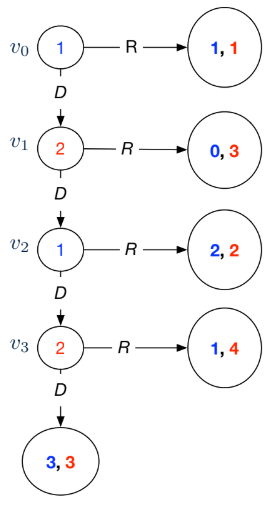
\includegraphics[width=0.4\textwidth]{images/centipede-game.png} 
    % \caption{$h(s)$ = number of misplaced tiles or sum of Manatten distances of each tile to their goal position}
    \label{fig:my_handwritten_notes}
\end{figure}
\noindent Based on Zermelo's Algorithm,
\begin{enumerate}
    \item At $v_3$, Player 2 chooses $R$, since 4>3.
    $v_3$ effectively becomes the payoff (1, 4).
    \item At $v_2$, Player 1 chooses $R$, since 2>1.
    $v_2$ effectively becomes the payoff (2, 2).
    \item At $v_1$, Player 2 chooses $R$, since 3>2.
    $v_1$ effectively becomes the payoff (0, 3).
    \item At $v_0$, Plyaer 1 chooses $R$, since 1>0.
    $v_0$ effectively becomes the payoff (1, 1).
\end{enumerate}
Based on backward induction, when both players are perfectly rational and can predict each other's moves,
Player 1 just chooses $R$ and stops the game.\newline
The paradox is that they could each have had a greater payoff of (3, 3) if they trusted each other (deviating from the rational path) 
and played $D$ all the way.

\newpage

\section{Minimax Search}
\begin{algorithm}[H]
\caption{Minimax search}
\SetKwFunction{Fback}{backpropagate}
\SetKwProg{Fn}{function}{}{end function}

$done \leftarrow leaves((S, E))$\;
\While{$done \neq S$}{
    $next \leftarrow \{s' \in S \setminus done \mid children(s', (S, E)) \subseteq done\}$\;
    \For{$s \in next$}{
        $C \leftarrow children(s, (S, E))$\;
        \If{$owner(s) = 1$}{
            $O \leftarrow \arg \max_{s' \in C} u(s')$ \tcp*[r]{maximise}
        }
        \Else{
            $O \leftarrow \arg \min_{s' \in C} u(s')$ \tcp*[r]{minimise}
        }
        $s'' \leftarrow$ any element of $O$\;
        $u(s) \leftarrow u(s'')$ \tcp*[r]{back score up}
        $done \leftarrow done \cup \{s\}$\;
    }
}
\end{algorithm}
\begin{Verbatim}
# Minimax search
done ← leaves((S, E))
while done ≠ S:
    next ← { s' ∈ S ∖ done | children(s', (S, E)) ⊆ done }
    for s ∈ next:
        C ← children(s, (S, E))
        if owner(s) = 1:
            O ← arg max_{s' ∈ C} u(s')        # maximise
        else:
            O ← arg min_{s' ∈ C} u(s')        # minimise
        s'' ← any element of O
        u(s) ← u(s'')                         # back score up
        done ← done ∪ {s}
\end{Verbatim}

\begin{itemize}
    \item Here, we are concerned with zero sum games, which are a subset of extended form games.
    \item For a two player zero sum game (where one player's win is the other player's loss)
    \[G = (N = \{1, 2\},\: (S, E, s_0),\: owner,\: a,\: u)\]
    \begin{itemize}
        \item The components are almost the same as extended form games, except:
        \item $N = \{1,2\}$ is set of two players
        \item $u: leaves((S, E))\rightarrow \{1,-1\}$ gives the scores for player 1.
        The score of player 2 is the negation of score of player 1. 
    \end{itemize}
    \item Minimax is a variation of backward induction, optimised for zero sum games.
\end{itemize}

\subsection{Depth-limited minimax with heuristics} In practice, real game trees are too large for full backward induction.
We want to use depth-limited search. We then have to replace the exact utilities at new leaves with some heuristic evaluations.
For example, in chess it might be $h(s) = 9Q + 5R + 3B$.

\subsection{Alpha-beta pruning}
An optimisation for minimax. 
\begin{figure}[H]
    \centering
    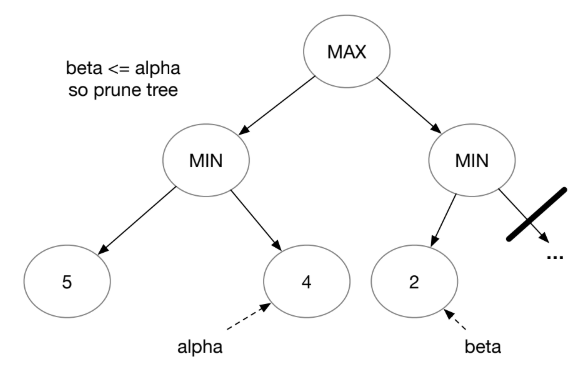
\includegraphics[width=0.8\textwidth]{images/alpha-beta-pruning.png} 
    % \caption{$h(s)$ = number of misplaced tiles or sum of Manatten distances of each tile to their goal position}
    \label{fig:my_handwritten_notes}
\end{figure}
\begin{itemize}
    \item Keep track of $\alpha$, the best (highest) value that Maximiser has found so far.
    \item $\beta$ is the lowest value that Maximiser has found so far.
    \item If $\beta \leq \alpha$, stop searching a branch. There is no point as Maximiser cannot get a higher value $\alpha$.
\end{itemize}


\end{document}